\section{Schwarz-SEM framework}
\label{section:schwarz-SEM_framework}
Because we intend to simulate nonspherical spinning bodies, it becomes necessary to create two different meshes. We create one circular mesh which conforms to the shape of the body and rotates with the body, as Fig. \ref{fig:mesh} shows. We utilize another static, background mesh with a circular cavity where the circular mesh is placed. There is an overlap between the two meshes to allow for data exchange. We utilize the Schwarz-spectral element method (Schwarz-SEM) framework, which allows us to run simulations with multiple meshes. The Schwarz-SEM framework has its roots in the Overlapping-Schwarz (OS) methods developed by Schwarz in 1870 \cite{mittal_nonconforming_2019}. Laplace's equation was solved on two overlapping domains by interpolating interdomain boundary conditions.  

\begin{figure}\centerline{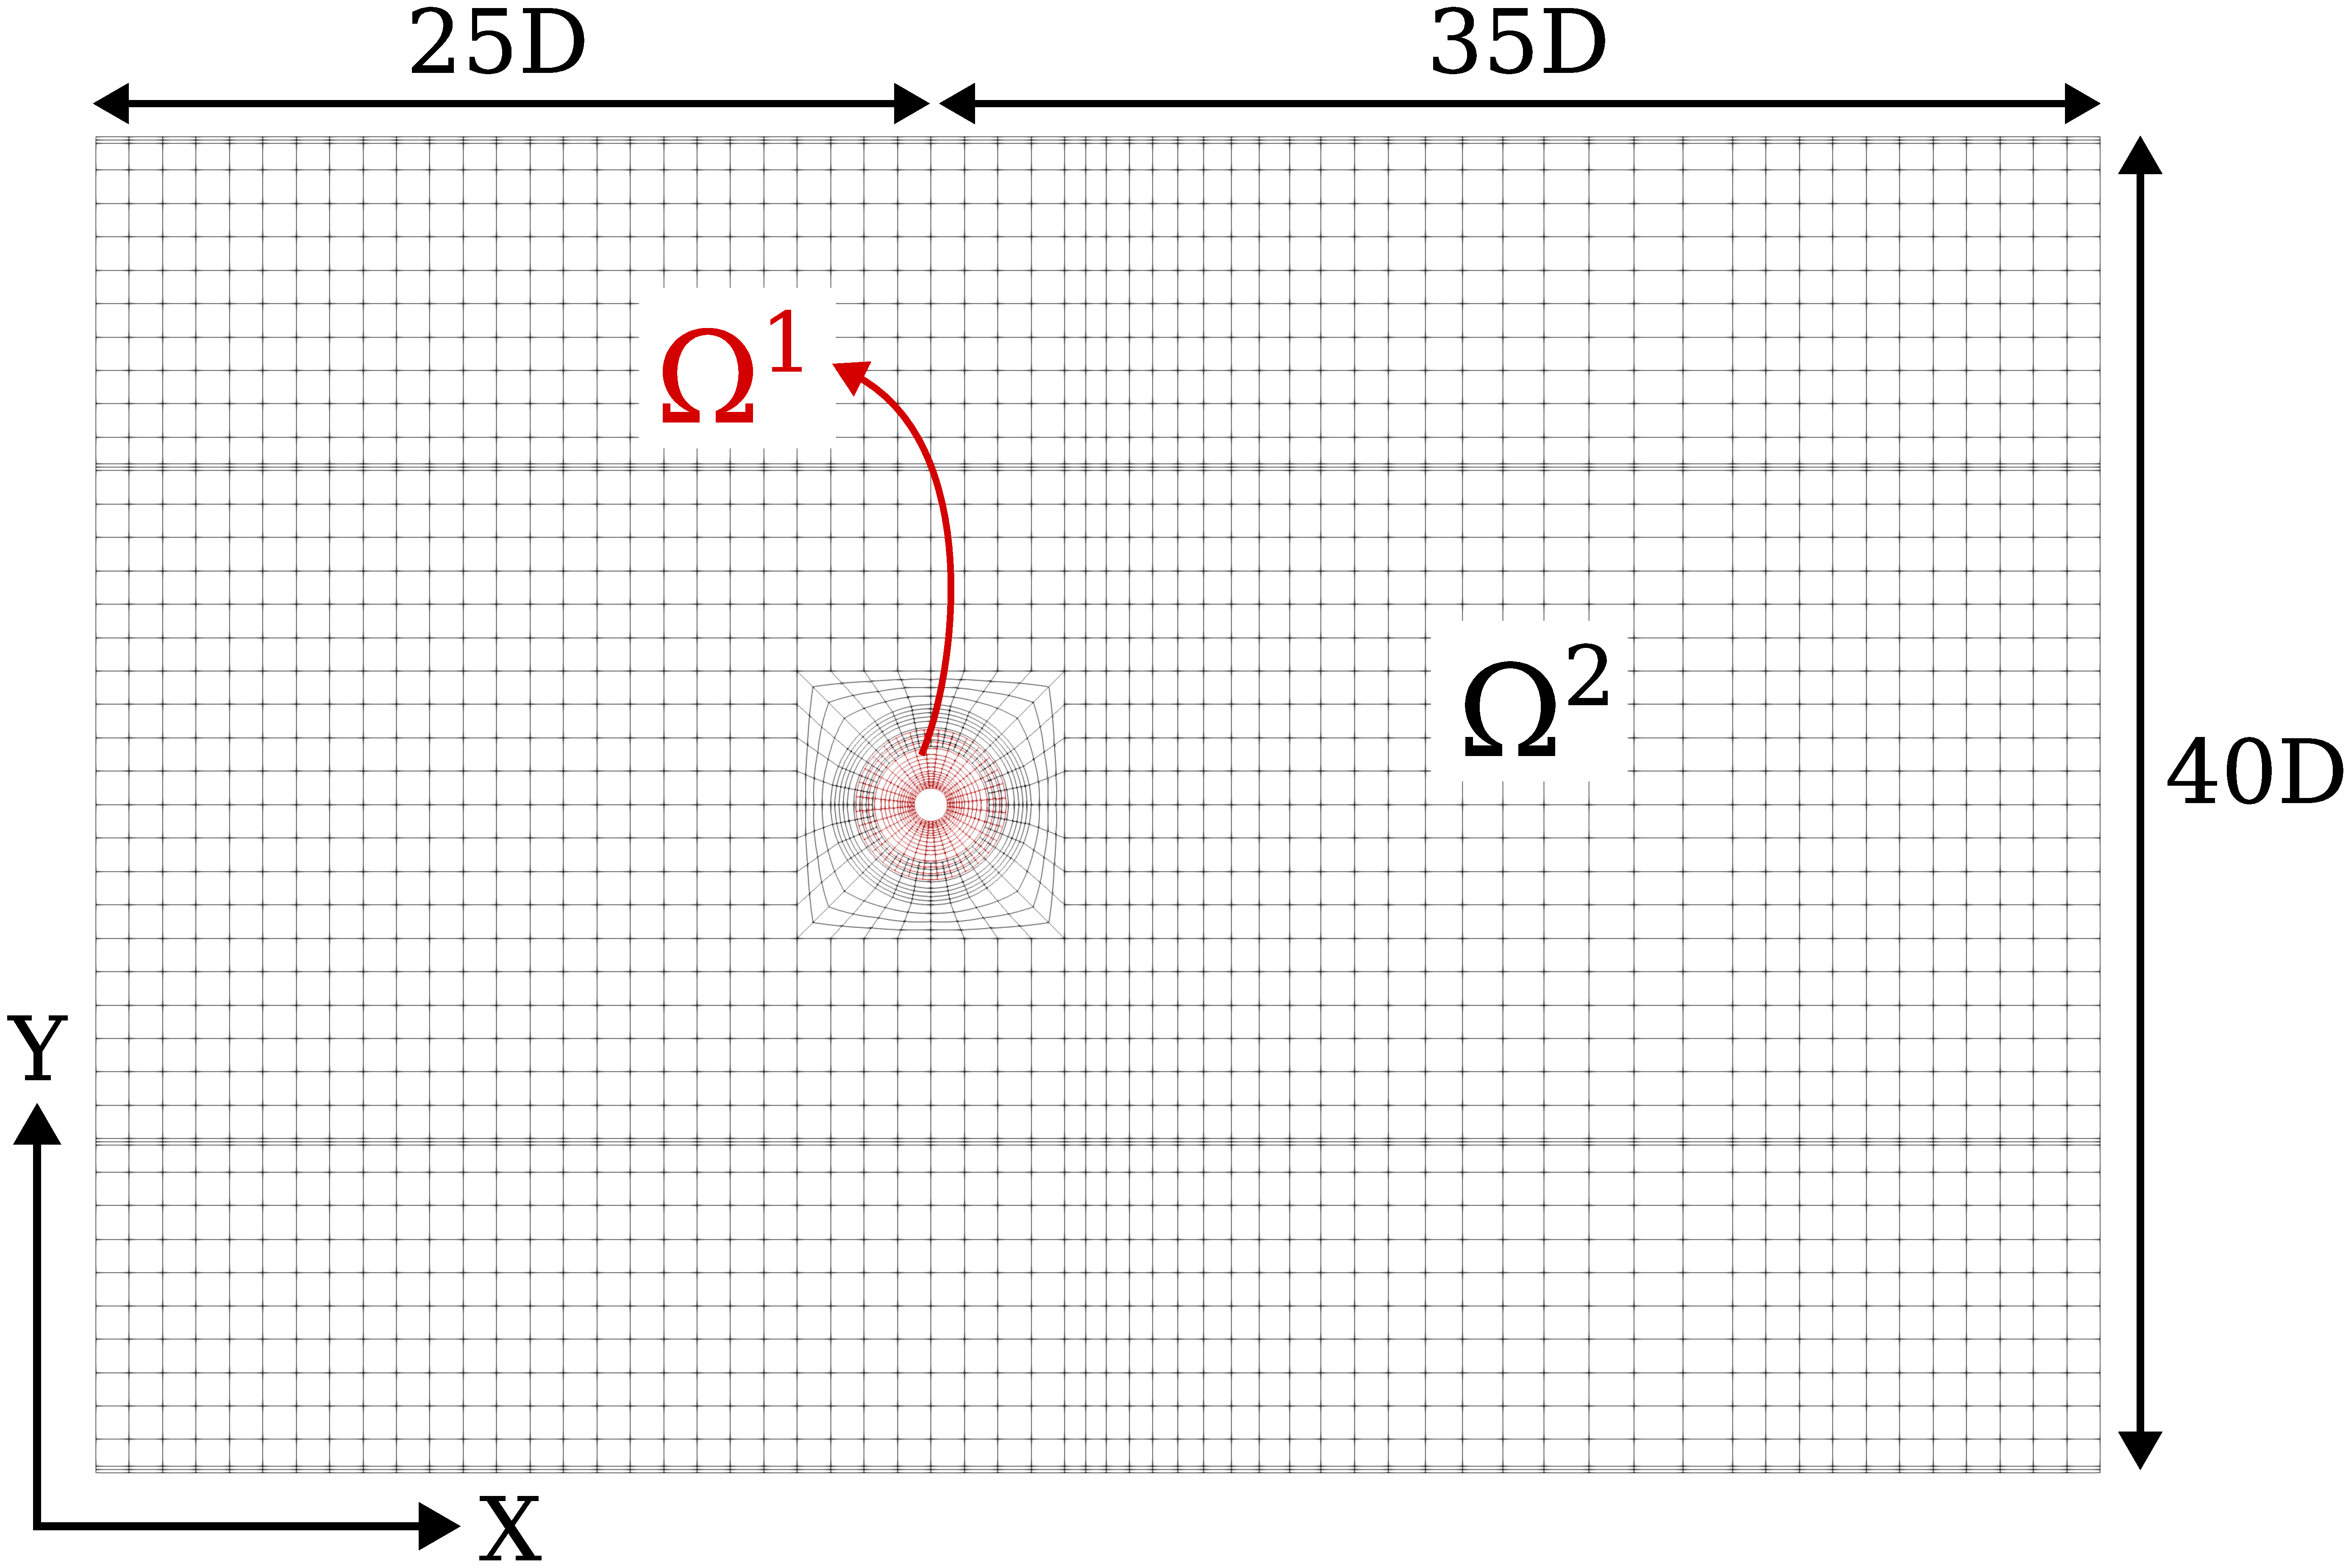
\includegraphics[width=.8\textwidth]{mesh.eps}}
    \caption{A figure showing the two meshes $\Omega^1$ and $\Omega^2$ in the Schwarz-SEM framework}
    \label{fig:mesh}
\end{figure}

In spite of the fact that the Schwarz-SEM framework was developed with the intention for use in static domains, an Arbitrary Lagrangian-Eulerian (ALE) formulation has been developed to allow for moving bodies. The implementation of the ALE formulation occurs with a modification of the convective term in Equations \ref{eq:INSE} and \ref{eq:density transport} \cite{merrill_moving_2019}. The advantage of using an overlapping mesh rather than a sliding mesh is we are able to retain spectral accuracy; sliding mesh methods are limited to second-order accuracy.

For advancing in time, a semi-implicit scheme is implemented, rather than a fully implicit scheme. The justification for choosing a semi-implicit scheme is the cost of a fully implicit scheme \cite{tomboulides_numerical_1997}. In the semi-implicit scheme, the nonlinear terms and Boussinesq forcing term are treated explicitly with \textit{k}th-order extrapolation since they would increase the cost substantially if treated implicitly. The time derivative is implicitly treated with a \textit{k}th-order backward difference formula (BDF\textit{k}) to retain high-order temporal accuracy. The viscous and pressure terms are decoupled and treated implicitly through Poisson updates.

Every timestep, the boundary conditions at the interdomain boundaries are interpolated from the adjacent mesh. This occurs every timestep because the locations of the inner mesh GLL nodes change every timestep. Mittal et al. \cite{mittal_nonconforming_2019} implemented a routine called \textit{findpts\_eval} from the library \textit{gslib} that carries out the boundary condition interpolation. Using the \textit{findpts} routine, the routine \textit{findpts\_eval} finds the corresponding element and element coordinates from the adjacent mesh.

At the interdomain boundaries, the solutions are advanced in time every timestep with EXT\textit{m} using $m$ number of preceding steps in time to increase the temporal accuracy. Higher order $m$ leads to instability, so $q$ corrector iterations are implemented every timestep, and the data is interpolated from the adjacent domain before every corrector iteration. In the case of our parameter sweep, we set $m=3$ and $q=5$ to achieve sufficient data exchange.
  
The top and bottom boundaries have symmetric boundary conditions. The left boundary has a Dirichlet constant-velocity inflow boundary condition, while the right boundary has a Neumann zero-pressure outflow boundary condition. Meanwhile, the surface of the cylinder has a Dirichlet no-slip wall boundary condition. The size of the domain is $60D \times 40D$, where $D$ is the length of the nonvarying axis of the ellipse; the radius of the inner mesh is $2.25D$. The inner mesh consists of 512 elements, while the outer mesh consists of 3200 elements. There is an overlap of $0.5D$ between the meshes. 

